\documentclass[12pt,german]{article}
\usepackage{listings}
%\usepackage[utf8]{inputenc}
\usepackage{inputenc}
\usepackage{graphicx}
\usepackage{float}
\usepackage{array}
\usepackage{pdfpages}

\lstset{
extendedchars=\true,
language=JAVA,
numbers=left, 
numberstyle=\footnotesize, 
%inputencoding=utf8,
%basicstyle=\ttfamily,
%basicstyle=\ttfamily\fontsize{8}{8},
%commentstyle=\ttfamily\fontsize{8}{8},
basicstyle=\tiny;
columns=fullflexible,
%xleftmargin=5pt,
frame=single,
breaklines=true,
postbreak=\mbox{{$\hookrightarrow$}\space},
}
\renewcommand{\thesubsubsection}{\alph{subsubsection} )}
%\renewcommand{\thesubsubsection}{\thesubsection.\alph{subsubsection} )}

\setcounter{section}{2}

\begin{document}

\title{Übungsaufgaben III, SBV1 }
\author{Lukas Fiel, Lisa Panholzer}
\maketitle


\newpage
\section{Übungsaufgaben III}
\subsection{Resampling und Bildüberlagerung}
\subsubsection{Zerteilen eines Bildes}
\label{chopImg}
Zur vertikalen Teilung eines Bildes wurde ein simpler Filter \textit{ChopImgInHalf\_} in \textit{ImageJ} implementiert. Dieser definiert zuerst eine ROI (region of interest) welche die erste Hälfte des Bildes beinhaltet. Mittels \textit{ImageJUtility.chopImage} kann dieser Bereich aus dem Ursprungsbild herausgeschnitten und angezeigt werden. Die Berechnung der zweiten Hälfte des Bildes unterscheidet sich lediglich durch die linke obere Koordinate des interessanten Bereichs (ROI). 

\begin{table}[H]
  \centering
  \begin{tabular}{| c | c | c |}
	\hline
	 & erste & zweite \\	
	Testbild & Bildhälfte & Bildhälfte \\ 
    \hline
    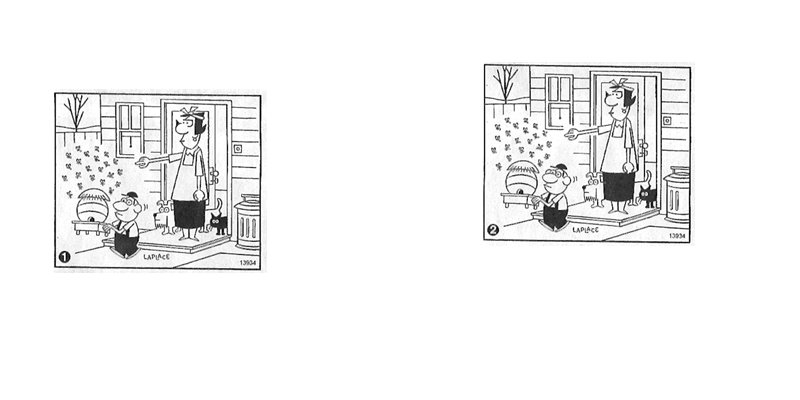
\includegraphics[width=5cm]{images/chop/binary1.jpg} &
    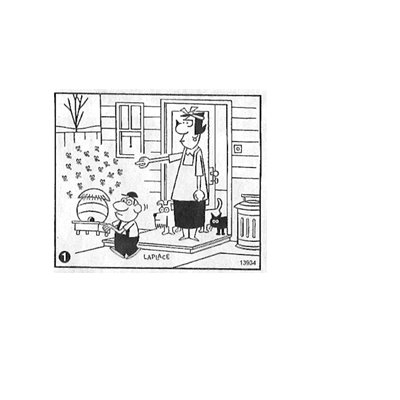
\includegraphics[width=2.5cm]{images/chop/binary1FH.jpg} &
    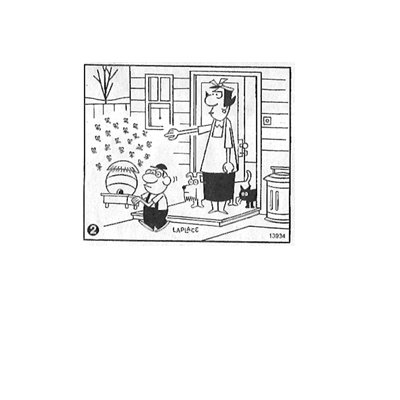
\includegraphics[width=2.5cm]{images/chop/binary1SH.jpg} \\
    \hline
    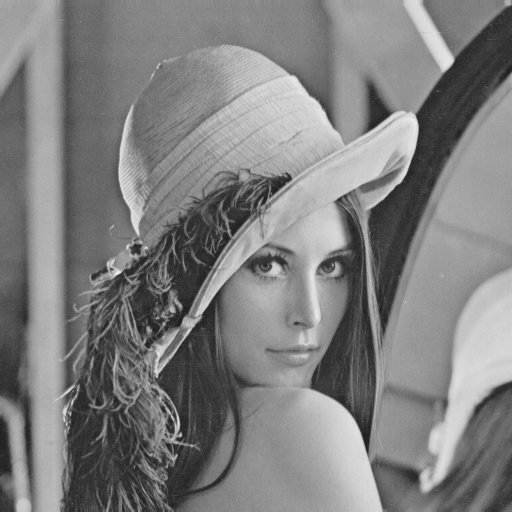
\includegraphics[width=5cm]{images/chop/lena.jpg} &
    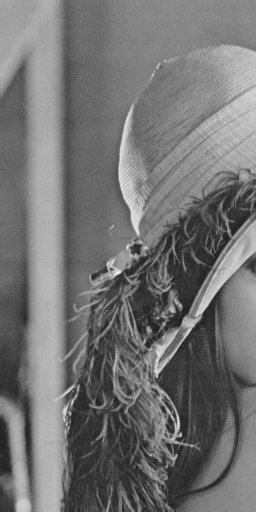
\includegraphics[width=2.5cm]{images/chop/lenaFH.jpg} &
    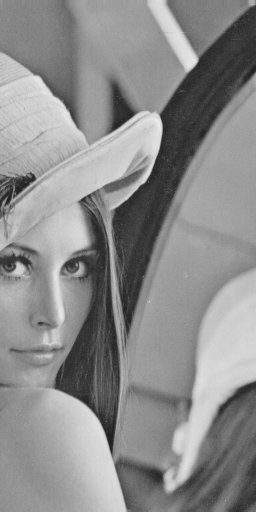
\includegraphics[width=2.5cm]{images/chop/lenaSH.jpg} \\
    \hline
    
  \end{tabular}
  \caption{Zerteilung eines Bildes anhand selbst definiertem Filter}
  \label{tab:chopInHalfTest}
\end{table}

\lstinputlisting[frame=single,language=JAVA,breaklines=true]{../../ChopImgInHalf_.java}




\subsubsection{Transformation mittels Nearest Neighbor und Bilinearer Interpolation}

In einem separaten Filter \textit{RegisterFinal\_.java} wurden die Funktionalitäten implementiert, die für die automatische Registrierung in c) benötigt werden. Bei Aufruf des Filters wird als erstes die Funktionalität des \textit{ChopImgInHalf\_.java} Filter angewandt. Diese sorgt dafür, dass das Eingangsbild in zwei Hälften geteilt und das Originalbild A von Bild B getrennt wird. Abschließend werden neben dem bereits geöffneten Originalbild die zwei getrennten Bildhälften ausgegeben. Die Neuberechnung der Bilder erfolgt entweder mit der Nearest Neighbor- oder der Bilinearen Interpolation. Hierzu wurde eine boolsche Variable als Flag definiert, die je nach Wert eine der beiden Interpolationsmethoden verwendet.

Anschließend müssen deltaX und deltaY für die Translation angegeben werden. Für die Rotation muss zusätzlich noch der Rotationswinkel angegeben werden. Nach dem der User die Eingaben  getätigt und bestätigt hat, wird das Bild B dementsprechend neu positioniert und gedreht.

Anbei folgen Testbilder, die die Funktionalität wiederspiegeln:

\begin{table}[H]
  \centering
  \begin{tabular}{| c | c | c | c |}
	\hline
	gegebenes & erste & zweite & resultierendes \\	
	Testbild & Bildhälfte & Bildhälfte & Ergebnis \\ 
    \hline
     & & & \\
    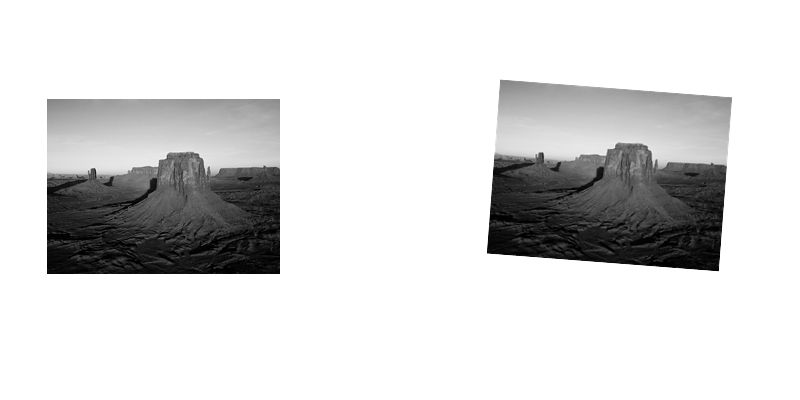
\includegraphics[width=5cm]{images/register/gray1.jpg}  &
    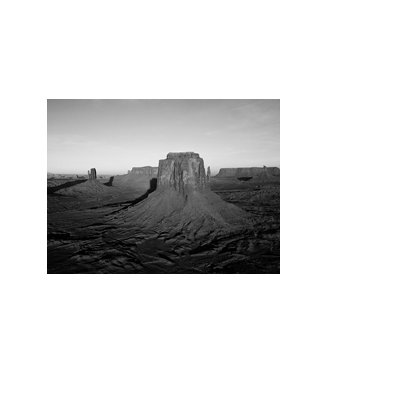
\includegraphics[width=2.5cm]{images/register/first-half-image-01.jpg} &
    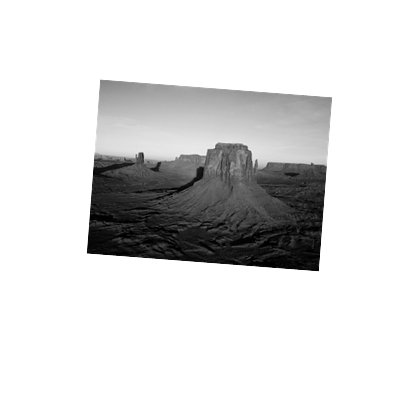
\includegraphics[width=2.5cm]{images/register/second-half-image-01.jpg} &
    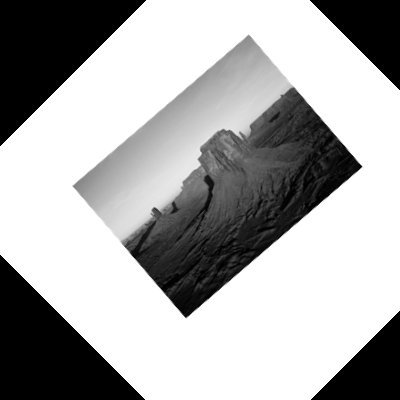
\includegraphics[width=2.5cm]{images/register/transformed-image-01.jpg} \\
    
	deltaX=20, deltaY=20, & & & \\
	rotation=45, nnFlag=false & & & \\
    
    
    \hline
     & & & \\
    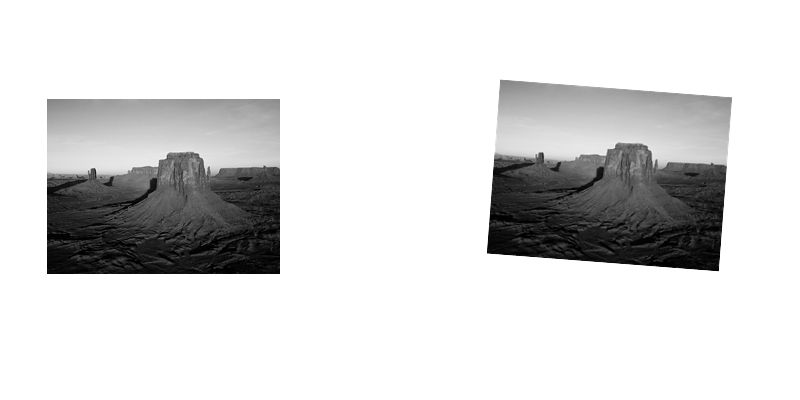
\includegraphics[width=5cm]{images/register/gray1.jpg}  &
    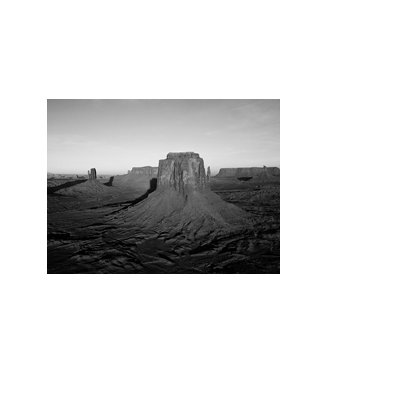
\includegraphics[width=2.5cm]{images/register/first-half-image-01.jpg} &
    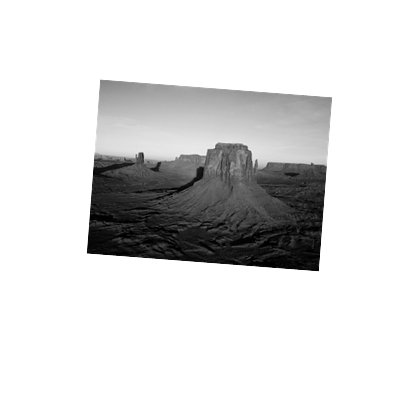
\includegraphics[width=2.5cm]{images/register/second-half-image-01.jpg} &
    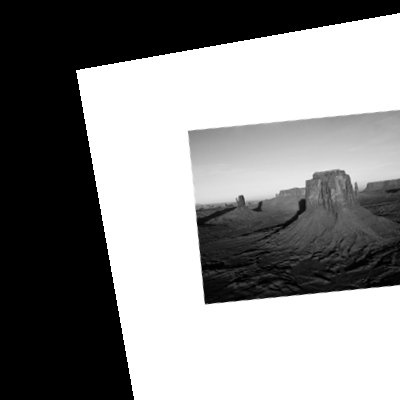
\includegraphics[width=2.5cm]{images/register/transformed-image-02.jpg} \\
    deltaX=100, deltaY=50, & & & \\
    rotation=10, nnFlag=false  & & & \\
    
    
    \hline
     & & & \\
    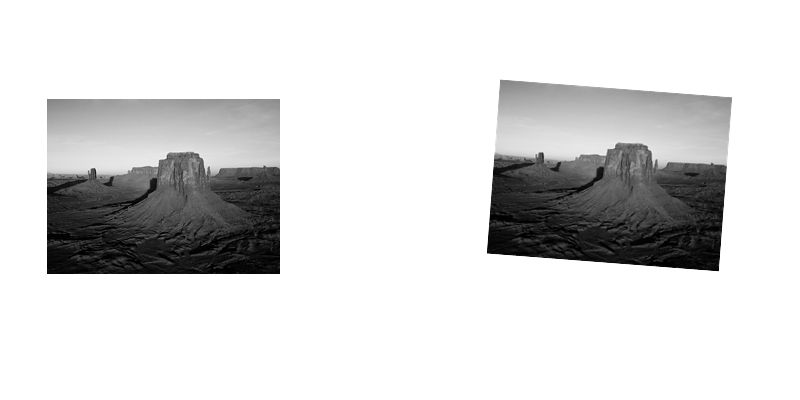
\includegraphics[width=5cm]{images/register/gray1.jpg}  &
    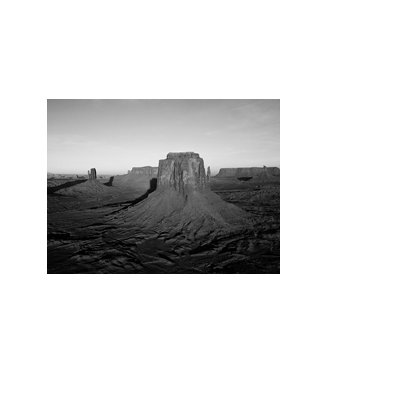
\includegraphics[width=2.5cm]{images/register/first-half-image-01.jpg} &
    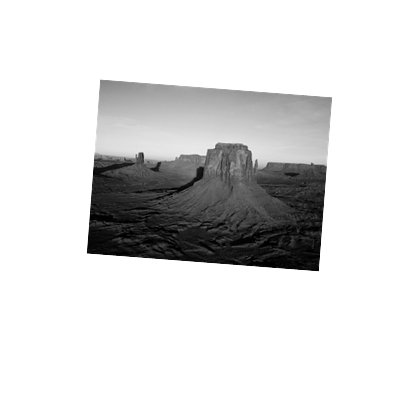
\includegraphics[width=2.5cm]{images/register/second-half-image-01.jpg} &
    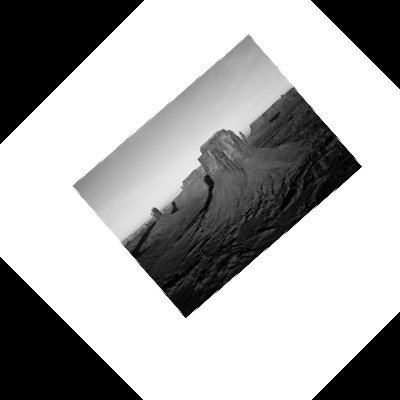
\includegraphics[width=2.5cm]{images/register/transformed-image-03.jpg} \\
	deltaX=20, deltaY=20,  & & & \\
	rotation=45, nnFlag=true & & & \\
    
    \hline
     & & & \\
    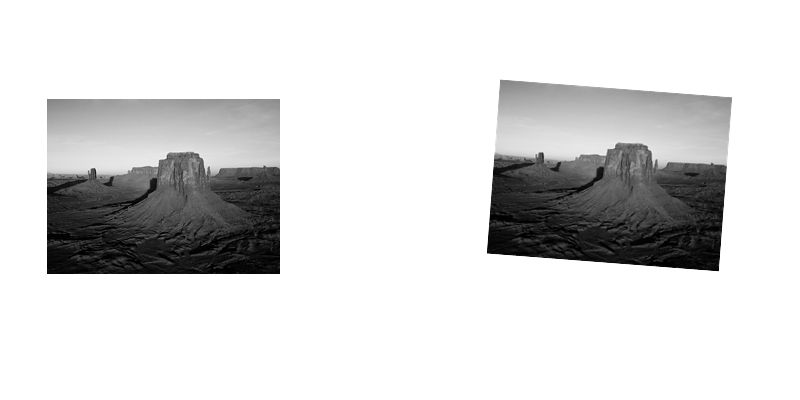
\includegraphics[width=5cm]{images/register/gray1.jpg}  &
    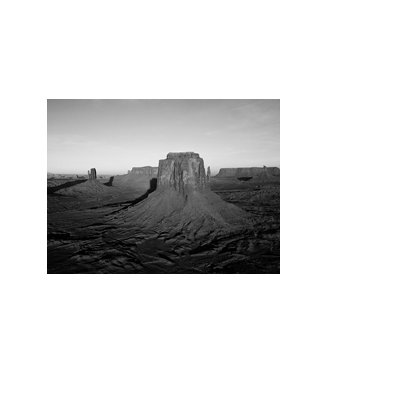
\includegraphics[width=2.5cm]{images/register/first-half-image-01.jpg} &
    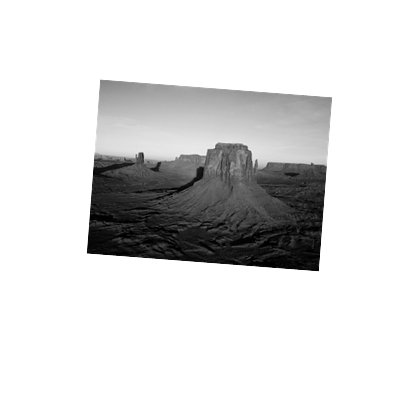
\includegraphics[width=2.5cm]{images/register/second-half-image-01.jpg} &
    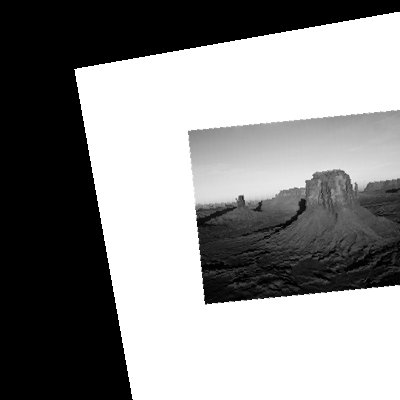
\includegraphics[width=2.5cm]{images/register/transformed-image-04.jpg} \\
    deltaX=100, deltaY=50,  & & & \\
    rotation=10, nnFlag=true  & & & \\
    \hline
    
  \end{tabular}
  \caption{Testfälle:Transformation mittels NN und Bilinearer Interpolation}
  \label{tab:registerTest}
\end{table}


\lstinputlisting[frame=single,language=JAVA,breaklines=true]{../../RegisterFinal_.java}

\subsubsection{Automatische Registrierung}
Es wurde ein Filter in \textit{ImgaeJ} implementiert, der zur automatischen Registrierung von Bildinhalten herangezogen werden soll. Dabei wurde von den gegebenen Testbildern ausgegangen. \\
Da diese mit einer Bildtiefe von $8 bit$ nur Werte von $0$ (schwarz) bis $255$ (weiß) aufweisen, kann mittels SSE einfach ein Algorithmus geschrieben werden, der die Bilder voneinander subtrahiert und die Pixelwerte des Resultatbildes als Fitness heranzieht und aufsummiert. Der Hintergrund der gegebenen Bilder ist dabei meist weiß ($255$). Bei einer Verschiebung und anschließender Subtraktion entstehen aus diesem Grund aber schwarze Fragmente am Rand. Dieser Umstand kann leicht eliminiert werden, indem das Ursprungsbild zu Beginn invertiert wird. So ist der Hintergrund schwarz ($0$). Kanten werden dementsprechend weiß ($255$) dargestellt. \\
Das invertierte Bild wird anschließend, wie in Punkt \ref{chopImg} beschrieben, zerteilt und die Einzelbilder dargestellt. \\
Die eigentliche Registrierung verschiebt nun Bild1 in x und y Richtiung und rotiert dieses auch um jeweils ein Inkrement. Jedes dieser transformierten Bilder wird nun von Bild2 abgezogen und erneut ein Fitneswert berechnet. Es ist davon auszugehen, dass ein schwarzer Hintergrund ($0$) abgezogen von einem schwarzen Hintergrund ($0$) wiederum $0$ ergibt. Werden allerdings weiße Pixel von schwarzem Hintergrund abgezogen, oder schwarzer Hintergrund von weißen Linien abgezogen, so erhält man Werte abweichend von $0$. Auch Negativwerte sind so denkbar, wesshalb diese Differenzwerte zum Quadrat genommen werden. Hierdurch sind Differenzwerte immer positiv.\\
Wird Bild1 irgendwann genau auf die Position geschoben an der sich Bild2 befindet so subtrahieren sich die weißen Linien im Idealfall zu $0$. So kann ein eindeutiger Fitnesswert errechnet werden, der sein Optimum bei $0$ findet.\\
Aus Ressourcengründen werden all die beschriebenen Berechnungen/Verschiebungen mit dem NearesNeighbor Algorithmus berechnet. Ist das Optimum gefunden wird anschließend nocheinmal die Transformation mit Bilinearer Interpolation berechnet und von Bild2 subtrahiert. Das Resultatbild wird zum Schluss für den User sichtbar dargestellt um den Erfolg des Filters zu veranschlaulichen. \\

\begin{table}[H]
  \centering
  \begin{tabular}{| c | c | c | c |}
	\hline
	gegebenes & invertierter & invertierter & resultierendes \\	
	Testbild & Bildausschnitt1 & Bildausschnitt2 & Differenzbild \\ 
    \hline
    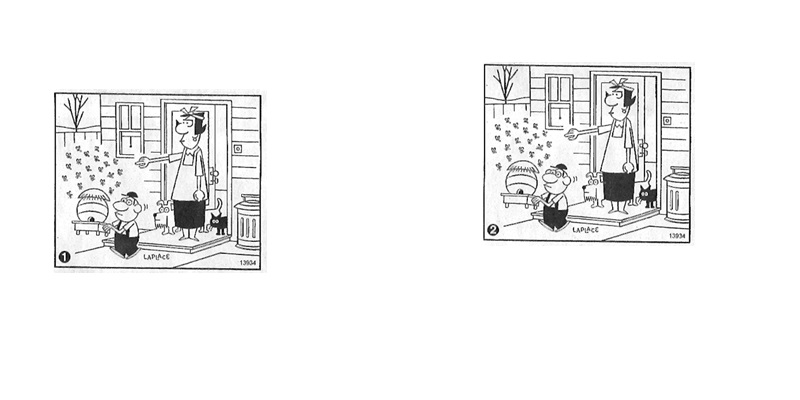
\includegraphics[width=5cm]{images/autoregister/binary1.jpg} &
    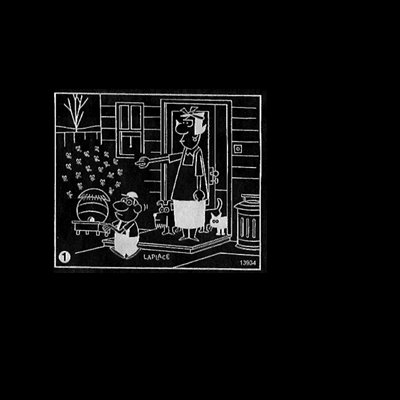
\includegraphics[width=2.5cm]{images/autoregister/binary1FH.jpg} &
    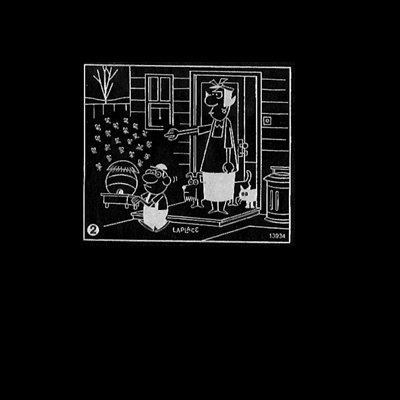
\includegraphics[width=2.5cm]{images/autoregister/binary1SH.jpg} &
    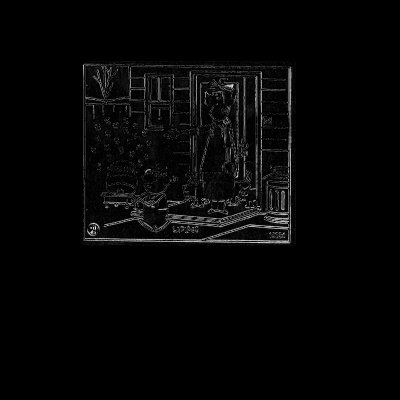
\includegraphics[width=2.5cm]{images/autoregister/binary1DIFF.jpg} \\
    \hline
    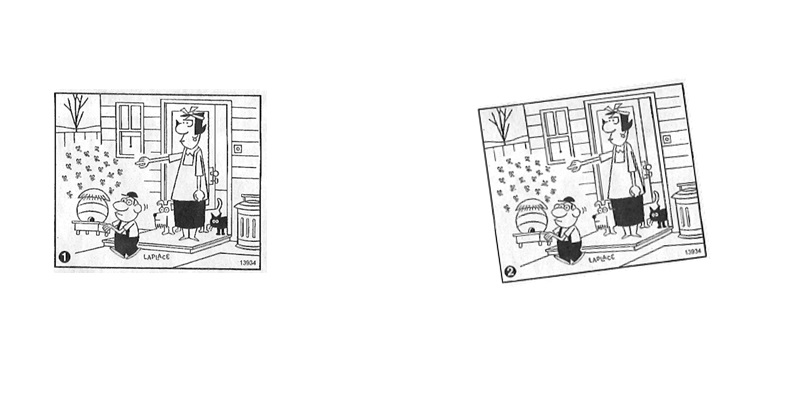
\includegraphics[width=5cm]{images/autoregister/binary2.jpg} &
    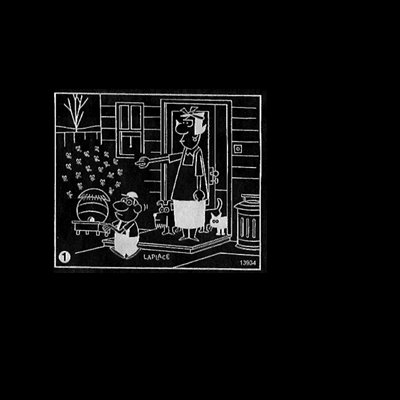
\includegraphics[width=2.5cm]{images/autoregister/binary2FH.jpg} &
    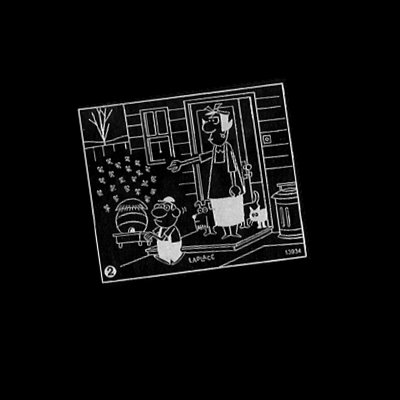
\includegraphics[width=2.5cm]{images/autoregister/binary2SH.jpg} &
    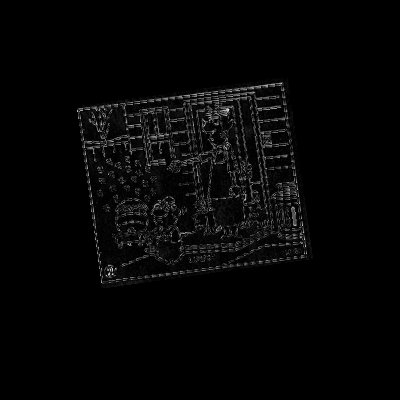
\includegraphics[width=2.5cm]{images/autoregister/binary2DIFF.jpg} \\
    \hline
    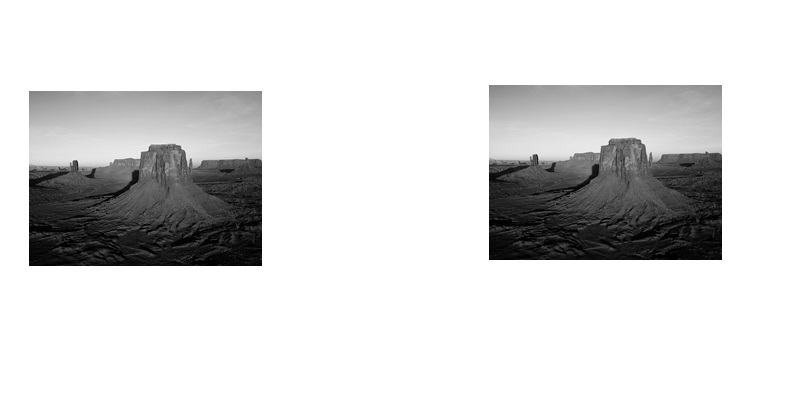
\includegraphics[width=5cm]{images/autoregister/gray2.jpg} &
    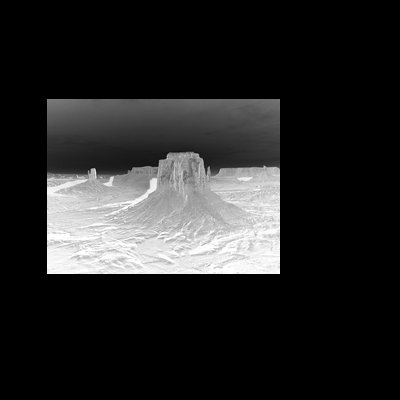
\includegraphics[width=2.5cm]{images/autoregister/gray1FH.jpg} &
    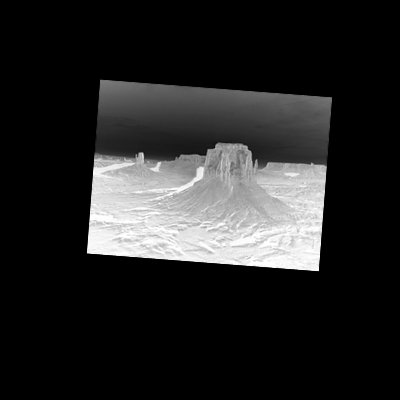
\includegraphics[width=2.5cm]{images/autoregister/gray1SH.jpg} &
    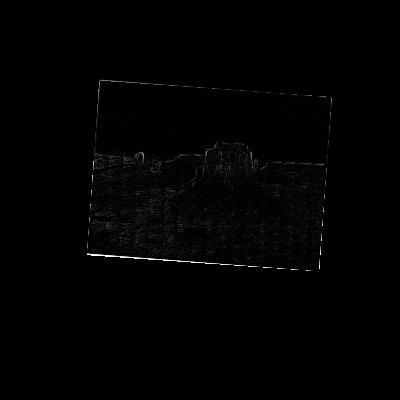
\includegraphics[width=2.5cm]{images/autoregister/gray1DIFF.jpg} \\
    \hline
    
  \end{tabular}
  \caption{Testfälle: automatische Registrierung}
  \label{tab:autoRegisterTest}
\end{table}

\lstinputlisting[frame=single,language=JAVA,breaklines=true]{../../AutoRegisterFinal_.java}

\end{document}
